\section*{Red con patrón (\emph{blazed grating})}

\item 
\begin{minipage}[t][2.5cm]{0.85\textwidth}
\textbf{Red de trasmisión con protuberancias con forma de prisma}
\begin{enumerate}
	\item Escriba la función transmisión para una red de rendijas de ancho $b$ y período $d$.
	\item (*) Ídem para una red formada por prismas delgados de alto $b$ y base $a$, con índice de refracción $n$, y separados por tramos obstruidos de alto $d-b$ (ver figura). 
\end{enumerate}
\end{minipage}
\begin{minipage}[c][1cm][t]{0.1\textwidth}
	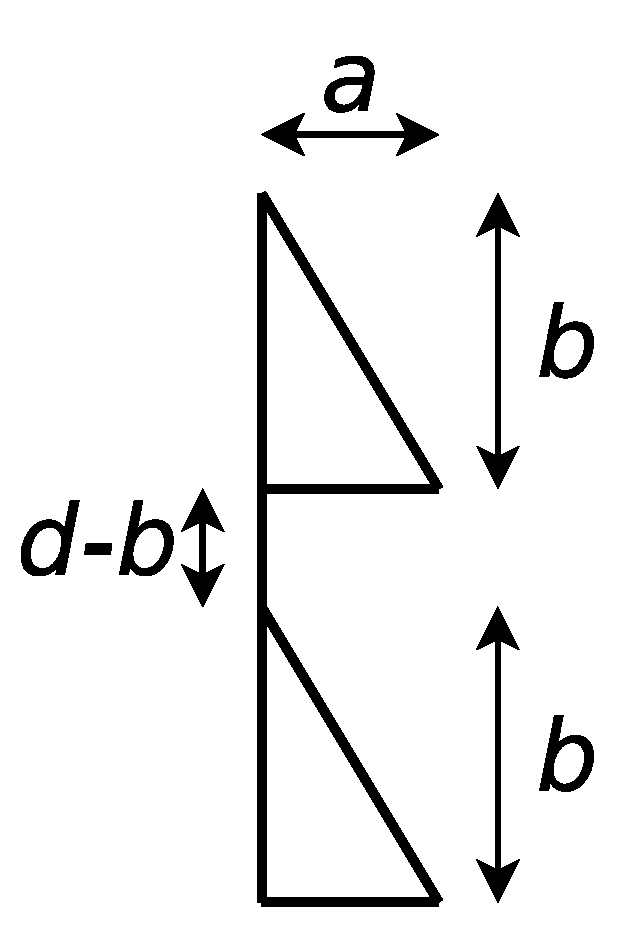
\includegraphics[width=\textwidth]{ej5-44}
\end{minipage}


\item (*) Una red de fase por reflexión tiene una densidad de facetas de \SI{4800}{\per\centi\metre} y ha sido construida para intensificar el primer orden, en $\lambda = \SI{0.6}{\micro\metre}$.
\begin{enumerate}
	\item Hallar el ángulo que forman las caras facetadas con el plano de la red. 
	\item Suponiendo incidencia normal, calcular la dispersión angular para esa $\lambda$. 
	\item Si se iluminase la red con $\lambda = \SI{0.48}{\micro\metre}$, ¿qué órdenes se verían?
\end{enumerate}

%\item 
%\begin{enumerate}
%	\item Hallar la distribución de irradianciaes sobre la pantalla para la red de transmisión descripta en el problema 13b).
%	La luz incide con un ángulo arbitrario sobre la red.
%	\item Comparar la distribución obtenida con la de una red de transmisión de $N$ rendijas de ancho $b$ y período $d$.
%	¿En qué se diferencian? 
%\end{enumerate}



\item
\begin{minipage}[t][3.5cm]{0.86\textwidth}
(*) Se tiene una red de difracción de $N$ períodos con una distribución de pares de prismas delgados de índices $n_1$, y $n_2$ y ángulos $\delta_1$ y $\delta_2$,
respectivamente, como muestra la figura.
Se la ilumina en forma normal.
Suponiendo que la teoría fuese exacta:
\begin{enumerate}
	\item Halle la irradiancia en la pantalla como función del ángulo $\theta$. 
	\item Elija parámetros de la red ($n_1$, $n_2$, $\delta_1$, $\delta_2$, $a$, $b$, $N$), para los cuales se intensifique el orden \num{-2} en el que se busca resolver las longitudes de onda de \SI{5000}{\angstrom} y \SI{5001}{\angstrom}.
\end{enumerate}
\end{minipage}
\begin{minipage}[c][0cm][t]{0.07\textwidth}
	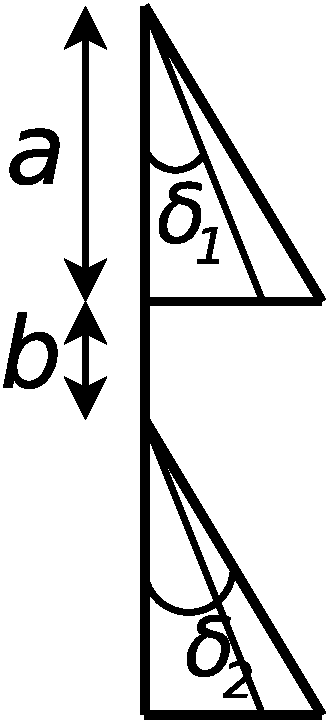
\includegraphics[width=\textwidth]{ej5-46}
\end{minipage}



\item (*) Una red de transmisión de ancho \SI{2}{\centi\metre} está formada por \num{50} prismas delgados.
Sabiendo que intensifica el segundo orden de interferencia, para $\lambda = \SI{5000}{\angstrom}$ calcule: 
\begin{enumerate}
	\item El ángulo del \emph{blaze}. 
	\item La posición angular del orden intensificado y de la imagen geométrica. 
	\item Discuta, en este caso, qué sucede con los otros órdenes de interferencia para la longitud de onda $\lambda$ dada.
	\item Calcule el poder resolvente para el segundo orden. 
\end{enumerate}
